\chapter{検出器量産と品質試験}
この章ではモジュールの組み立て工程と品質試験について説明する。

\section{組み立て工程}
モジュール組み立て機関は、初めにベアモジュールとフレキシブル基板を受け取る。
組み立て工程として以下が設定されている。
\begin{enumerate}
  \item フレキシブル基板・ベアモジュール貼り付け
  \begin{itemize}
    \item 受け取ったベアモジュールとフレキシブル基板を接着剤を用いて貼り付ける。
  \end{itemize}
  \item ワイヤー配線
  \begin{itemize}
    \item FEチップとフレキシブル基板を電気的に接続する。
  \end{itemize}
  \item ワイヤー保護
  \begin{itemize}
    \item ワイヤーが損傷があり断線が起きると、そのワイヤーに対するピクセルの読み出しができなくなるため、モジュールに屋根型の物質を取り付け、ワイヤーを物理的に保護する。
  \end{itemize}
  \item パリレンコーティング
  \begin{itemize}
    \item モジュール読み出し部以外での電通や放電を防ぐため、パリレン高分子を用いてモジュールを保護する。
  \end{itemize}
  \item 温度サイクル試験
  \begin{itemize}
    \item ITk運転時の環境温度は$-45^\circ$Cから$40^\circ$Cまで変化しうる\cite{3-2}。この温度変化に耐えうるかを確認するため、温度サイクルを行う。
  \end{itemize}
  \item 低温耐久試験
  \begin{itemize}
    \item ITk運転時の環境温度は$-40^\circ$C付近である。これに耐えうる性能を持つかを確認するために、低温下にモジュールを長時間設置する試験を行う。
  \end{itemize}
\end{enumerate}

流れと各組み立て工程のイメージを図\ref{assembly_flow}に示す。
\begin{figure}[bpt]\centering
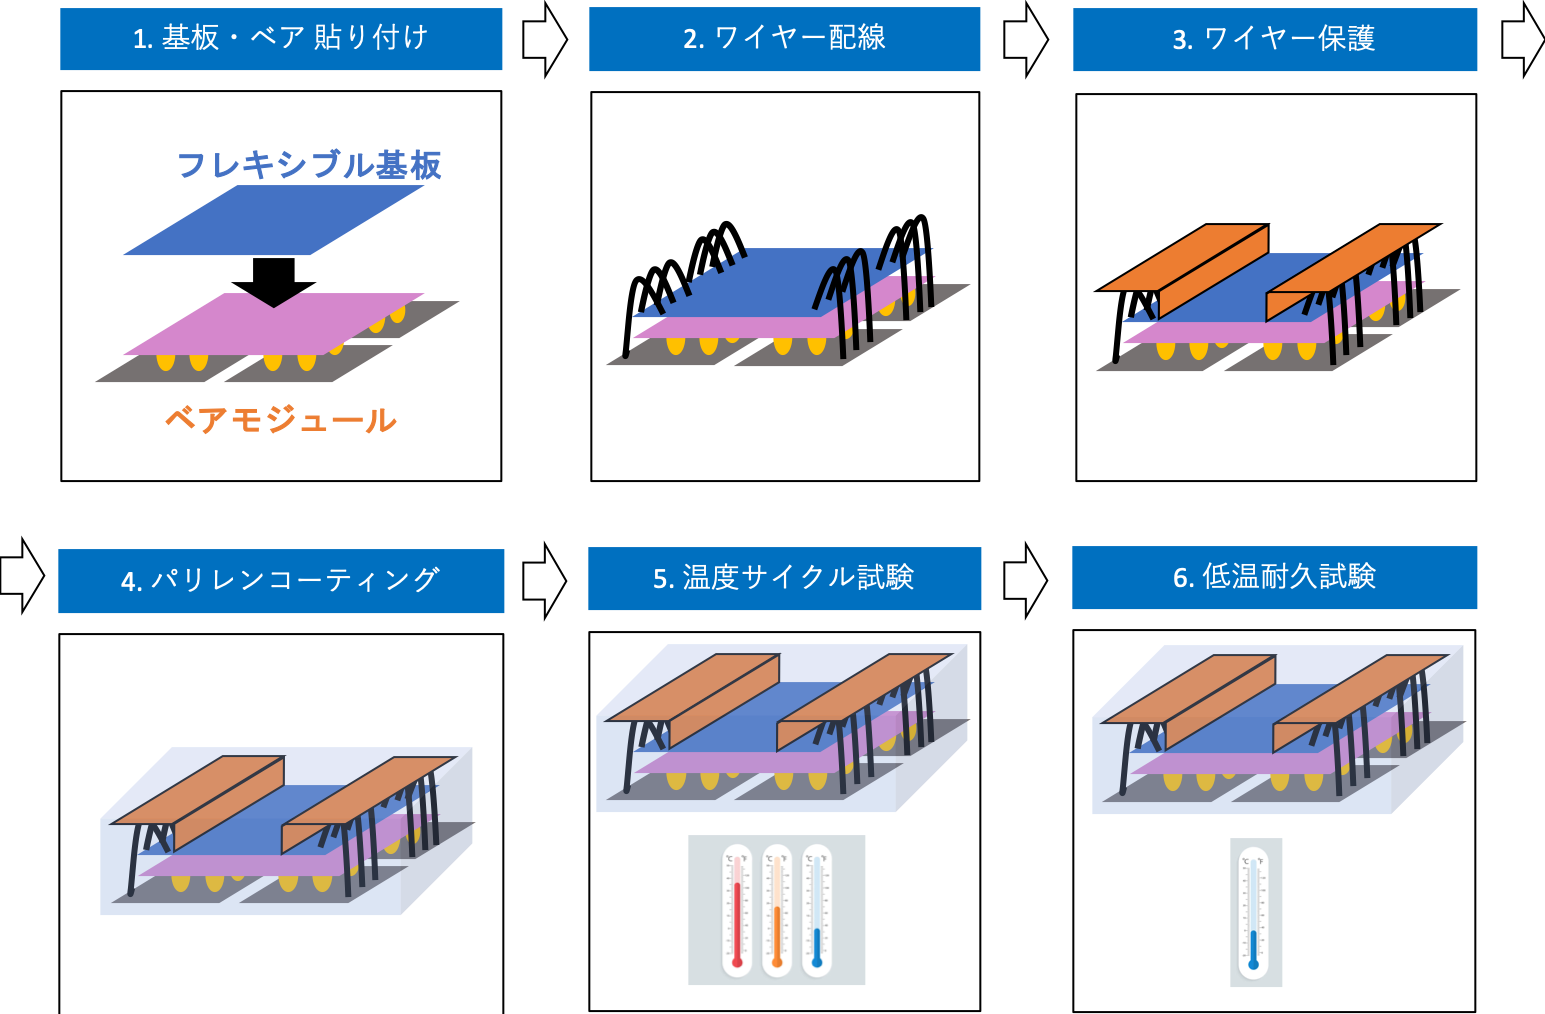
\includegraphics[width=14cm]{assembly_flow}
\caption[組み立て工程]{組み立て工程}
\label{assembly_flow}
\end{figure}

\section{品質試験}
各組み立て工程に対して、いくつかの品質試験を行う。行う品質試験の代表的なものを以下に示す。

\subsection{外観検査(Visual Inspection)}
モジュールの外観写真を撮り、モジュールに以下のような欠陥がないかを確認する。
また外観検査の様子を図\ref{VI_ovewview}に示す。
\begin{itemize}
  \item 抵抗等取り付け部品の損傷.
  \item ワイヤーの接着位置確認.
  \item 基板上の回路やワイヤーの断線.
  \item 付着汚れ.
\end{itemize}

\begin{figure}[bpt]\centering
  \begin{minipage}{0.4\hsize}
    \begin{center}
    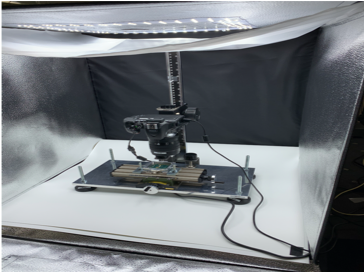
\includegraphics[width=60mm]{VI_setup}
    \end{center}
  \end{minipage}
  \begin{minipage}{0.4\hsize}
    \begin{center}
    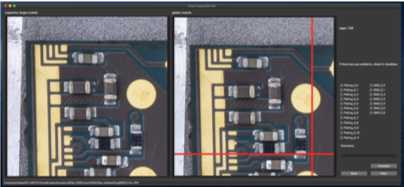
\includegraphics[width=65mm]{VI_analysis}
    \end{center}
  \end{minipage}
  \caption[外観検査の様子]{外観検査の様子}
  \label{VI_overview}
\end{figure}

\subsection{質量測定(Mass Measurement)}
モジュールの質量を測定。

\subsection{平坦性測定(Metrology)}
モジュール上の位置座標を相対的に何点か測定し、モジュールの平坦度、厚さ、歪み具合等を測定する。
測定の様子と解析の例を図\ref{Metrology_overview}に示す。

\begin{figure}[bpt]\centering
  \begin{minipage}{0.4\hsize}
    \begin{center}
    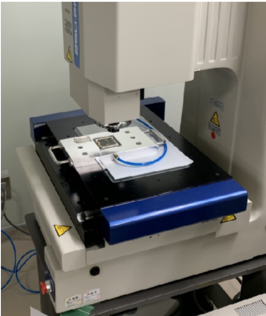
\includegraphics[width=60mm]{Metrology_setup}
    \end{center}
  \end{minipage}
  \begin{minipage}{0.4\hsize}
    \begin{center}
    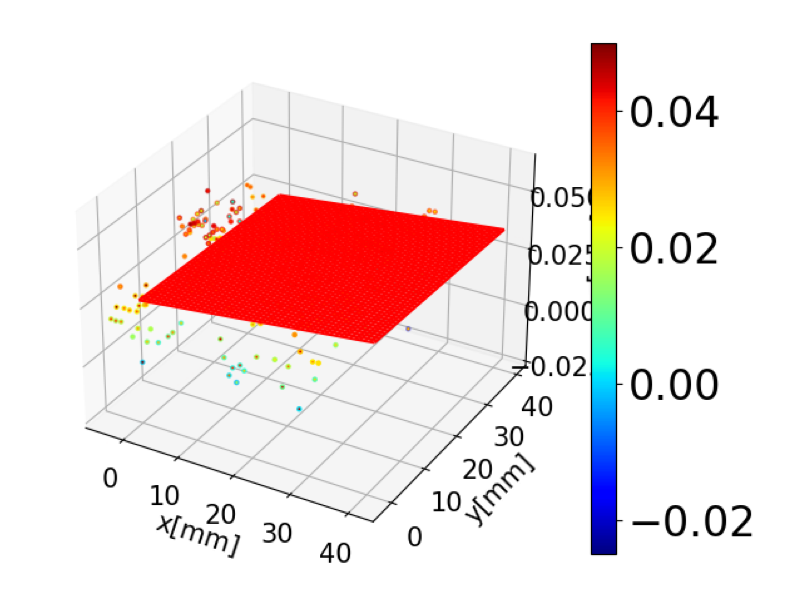
\includegraphics[width=65mm]{Metrology_analysis}
    \end{center}
  \end{minipage}
  \caption[平坦性測定の様子]{平坦性測定の様子}
  \label{Metrology_overview}
\end{figure}

\subsection{センサー電流-電圧特性確認(Sensor IV)}
モジュールのシリコンセンサーに逆バイアス電圧をかけ、電流-電圧特性をみる。
印加電圧を段階的に変化させて測定点をとり、電流と電圧の関係を確認する。
この試験の結果の例を図\ref{sensor_IV_result}に示す。
図\ref{pn_iv}に示すように、逆方向電圧では電流はほとんど流れないが、臨界電圧に達すると急激に増大する。

\begin{figure}[bpt]\centering
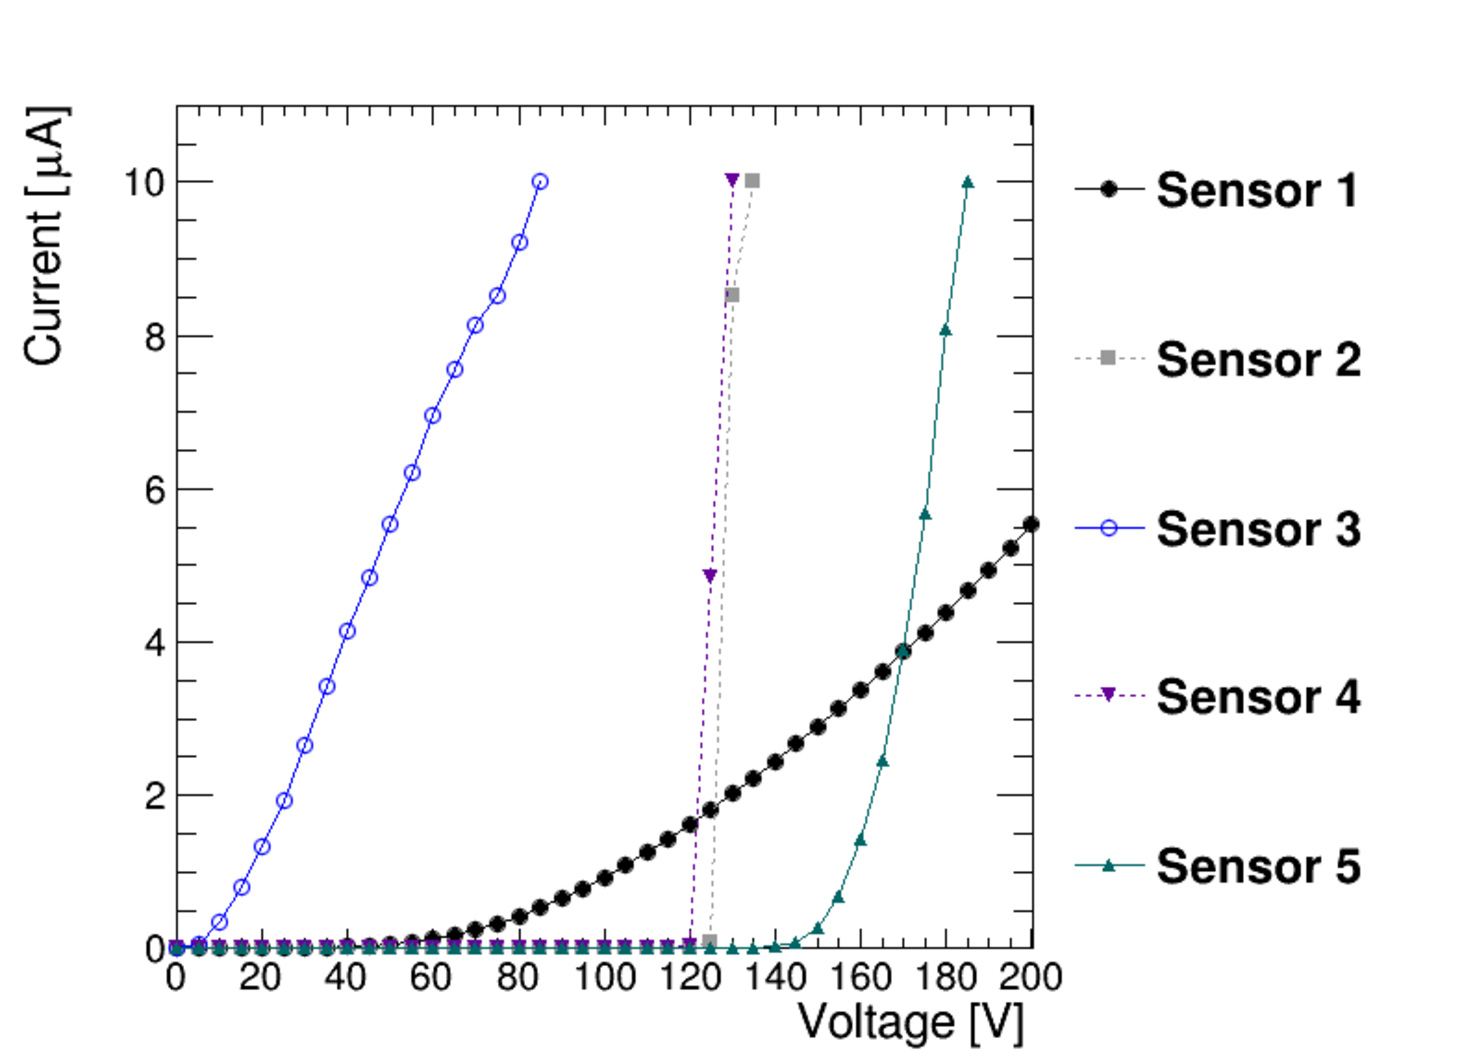
\includegraphics[width=14cm]{sensor_IV_result}
\caption[センサー電流-電圧特性結果の例]{センサー電流-電圧特性結果の例。}
\label{sensor_IV_result}
\end{figure}

\subsection{FEチップ電流-電圧特性確認(SLDO VI)}
FEチップに対して電圧をかけ、電流-電圧特性をみる。
センサーに対してと同様に、印加電圧を段階的に変化させて測定点をとり、電流と電圧の関係を確認する。
抵抗として振る舞うため、電流、電圧間の関係は図\ref{SLDO_VI_result}のように線形性を持つ。

\begin{figure}[bpt]\centering
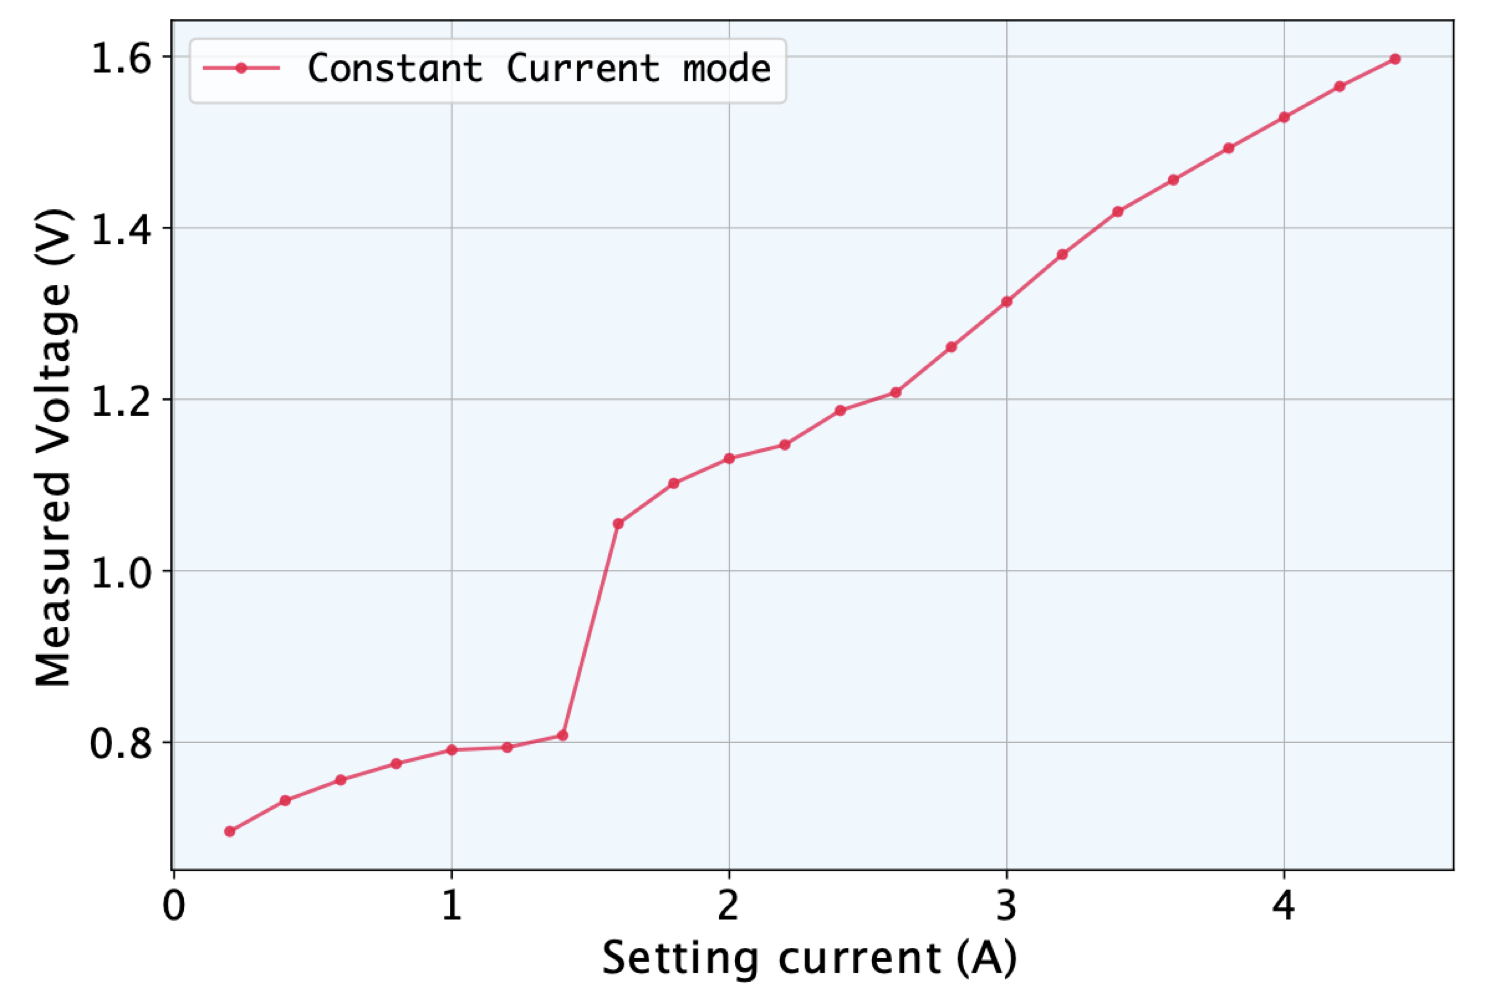
\includegraphics[width=14cm]{SLDO_VI_result}
\caption[FEチップ電流-電圧特性試験結果の例。]{FEチップ電流-電圧特性試験結果の例。}
\label{SLDO_VI_result}
\end{figure}

\clearpage
\subsection{読み出し試験}

\subsubsection{汎用読み出しシステムYARR}

\subsubsection{レジスタ書き換え(Chip Configuration)}

\subsubsection{試験項目詳細}
\begin{itemize}
  \item レジスタ読み出し(Register test)
  \item デジタル回路読み出し(Digital scan)
  \item アナログ回路読み出し(Analog scan)
  \item Threshold測定(Threshold scan)
  \item Thresholdグローバルレジスタ調整(Global threshold tuning)
  \item Thresholdピクセルレジスタ調整、再調整、精密調整(Pixel threshold tuning)
  \item ToTグローバルレジスタ調整(ToT tuning)
  \item ノイズ占有率測定(Noise scan)
  \item スタックピクセル測定(Stuck pixel scan)
  \item クロストーク測定(Crosstalk scan)
  \item バンプ接続確認測定(Disconnected bump scan)
  \item 外部トリガーを用いた測定(External trriger)
\end{itemize}
ここから1つ1つの詳細について説明する。
  
\subsubsection{Threshold調整とピクセル解析}\label{sec:pixel_analysis}
以下の流れで読み出しを行う。
\begin{itemize}
  \item デジタル回路読み出し
  \item アナログ回路読み出し
  \item Threshold測定
  \item Thresholdグローバルレジスタ調整
  \item Thresholdピクセルレジスタ調整
  \item ToTグローバルレジスタ調整
  \item Thresholdグローバルレジスタ再調整、精密調整
  \item Threshold測定
  \item スタックピクセル測定
  \item クロストーク測定
\end{itemize}

digital scan
・Explanation
・Output files


モジュール上のピクセルを解析し、各ピクセルが正常かどうかを判断する。
以下の評価基準で解析をし、不良ピクセルには評価基準に応じた評価名が付けられる

\begin{table}[tbp]
\begin{center}
\caption[ピクセル解析の評価基準]{ピクセル解析の評価基準\cite{3-1}}
\label{pixel_analysis_criteria}
  \begin{tabular}{|lll|} \hline
    評価名 & 読み出し項目 & 不良評価基準 \\ \hline
    Digital Dead      & Digital scan           & Occupancy < 1 \\ \hline
    Digital Bad       & Digital scan           & Occupancy < 98 or Occupancy > 102\\\hline 
    Merged Bump       & Analog scan            & Occupancy < 98 or Occupancy > 102 \\ 
                      & Crosstalk scan         & High Crosstalk\\ \hline
    Analog Dead       & Analog scan            & Occupancy < 1 \\ \hline
    Analog Bad        & Analog scan            & Occupancy < 98 or Occupancy > 102 \\ \hline
    Tuning Failed     & Threshold scan         & カイ二乗=0 \\ \hline
    Tuning Bad        & Threshold scan         & $\pm5\sigma$\\ 
                      & ToT scan               & 0 or 15 \\ \hline
    High ENC          & Threshold scan         & $\pm3\sigma$ \\ \hline
    Noisy             & Noise scan             & Occupancy > $10^{-6}$\\ \hline
    Disconnected Bump & Disconnected bump scan & 未決定 \\ 
                      & Source scan            & Occupancyが平均値の1$\%$ \\ \hline
    High Crosstalk    & Crosstalk scan         & Occupancy>0 with 25e(sync)\\
                      &                        & Occupancy>0 with 40e(lin and diff)\\ \hline 
  \end{tabular}
\end{center}
\end{table}

\subsubsection{簡易読み出し試験}
簡易読み出し試験では以下の項目を扱う。
\begin{itemize}
  \item レジスタ読み出し
  \item デジタル回路読み出し
  \item アナログ回路読み出し
  \item Threshold読み出し
  \item ToT読み出し
  \item バンプ接続確認読み出し
\end{itemize}

\subsubsection{バンプ接合確認試験(Bump bond quality)}
放射線源を用いてバンプ接合の確認を行う。

\subsection{各組み立て工程における品質試験}

各組み立て工程と品質試験項目を図\ref{stage_test_flow}に示す。
\begin{figure}[bpt]\centering

\includegraphics[width=10cm]{figure}
\caption[組み立て工程と対応する品質試験]{組み立て工程と対応する品質試験}
\label{stage_test_flow}
\end{figure}

\section{検出器量産と品質試験データ管理に対する要求}

読み出し試験については特にデータ管理が大変。

